% !TeX program = xelatex
% !TeX options = -shell-escape
% !TEX encoding = UTF-8

% --------------------------------------------------------------
% This is all preamble stuff that you don't have to worry about.
% Head down to where it says "Start here"
% --------------------------------------------------------------

\documentclass[12pt]{article}
\usepackage[margin=2cm]{geometry} % 頁面邊距設置
\usepackage{amsmath,amssymb,amsthm} % 數學相關套件
\usepackage{graphicx} % 圖形插入
\usepackage{booktabs} % 表格線條
\usepackage[AutoFakeBold,AutoFakeSlant]{xeCJK} % 中文支援
\usepackage{fancyhdr} % 頁首頁尾設置
\usepackage{xcolor,changepage,mdframed} % 顏色與框線相關
\usepackage{titlesec} % 標題格式
\usepackage{setspace} % 行距
\usepackage{minted} % 程式碼高亮（需安裝 Python 套件 pygments）
\usepackage{booktabs}
\usepackage{caption}
\usepackage{array}
\usepackage{ulem}
\usepackage[shortlabels]{enumitem} % 列表格式
\usepackage[colorlinks=true,linkcolor=black,urlcolor=blue,citecolor=blue]{hyperref}
% 超連結
\graphicspath{{images}}

% 字體設定 (xeCJK)
\setCJKmainfont{黑體-繁}
\setCJKmonofont{Noto Sans Mono CJK TC}

% 頁首/頁尾設定 (fancyhdr)
\pagestyle{fancy}
\fancyhead[L]{NASA Homework 11} % 可以用 \leftmark 取代
\fancyhead[R]{B13901011 吳亞倫}
\fancyfoot[C]{\thepage}
\renewcommand{\headrulewidth}{0.4pt}
\renewcommand{\footrulewidth}{0pt}
\setlength{\headheight}{15pt}

% tex-fmt: off
\newtheorem*{theorem}{Theorem}
\newenvironment{lemma}[2][Lemma]{\begin{trivlist}
\item[\hskip \labelsep {\bfseries #1}\hskip \labelsep {\bfseries #2.}]}{\end{trivlist}}
\newenvironment{exercise}[2][Exercise]{\begin{trivlist}
\item[\hskip \labelsep {\bfseries #1}\hskip \labelsep {\bfseries #2.}]}{\end{trivlist}}
\newenvironment{problem}[2][Problem]{\begin{trivlist}
\item[\hskip \labelsep {\bfseries #1}\hskip \labelsep {\bfseries #2}]}{\end{trivlist}}
\newenvironment{question}[2][Question]{\begin{trivlist}
\item[\hskip \labelsep {\bfseries #1}\hskip \labelsep {\bfseries #2.}]}{\end{trivlist}}
\newenvironment{corollary}[2][Corollary]{\begin{trivlist}
\item[\hskip \labelsep {\bfseries #1}\hskip \labelsep {\bfseries #2.}]}{\end{trivlist}}
\newenvironment{solution}{\begin{proof}[Solution]}{\end{proof}}
\newenvironment{answer}{\begin{proof}[Ans]}{\end{proof}}
\renewcommand{\thesubsection}{\thesection. (\alph{subsection})}

% 樣式設定

\setminted{frame=lines, linenos, framesep=2mm, breaklines=true, breakanywhere=true, autogobble=true}

% 自訂框線環境
\newmdenv[
  linewidth=2pt, linecolor=gray, backgroundcolor=gray!10,
  topline=false, bottomline=false, rightline=false,
  skipabove=10pt, skipbelow=10pt, innerleftmargin=10pt,
  innerrightmargin=0pt, innertopmargin=5pt, innerbottommargin=5pt
]{myquote}

\newenvironment{mycolorbox}[1][gray]{
  \renewmdenv[
    linewidth=2pt, linecolor=#1, backgroundcolor=#1!10,
    topline=false, bottomline=false, rightline=false,
    skipabove=10pt, skipbelow=10pt, innerleftmargin=10pt,
    innerrightmargin=0pt, innertopmargin=5pt, innerbottommargin=5pt
  ]{myquote}
  \begin{myquote}
}{\end{myquote}}

\linespread{1.1}
% \usemintedstyle{xcode}
\AtBeginEnvironment{minted}{\vspace{-10pt}} % 可根據需求調整間距數值
\setminted{breaklines=true, breakanywhere=true, autogobble=true}

% tex-fmt: on
\begin{document}
\thispagestyle{fancy}

%------------------------------------------------------------
%                         Start here
% -----------------------------------------------------------

\begin{center}
  {\large \bfseries Network Administration / System Administration} \\
  \vspace{1em}
  {\Large \bfseries Homework 11} \\
\end{center}

\vspace{2em}

\begin{tabular}{@{}l l}
  \textbf{Student:} & 吳亞倫 \\
  \textbf{ID:} & B13901011  \\
  \textbf{Department:} & 電機工程學系
\end{tabular}
\bigskip

\begin{mycolorbox}[cyan]
  \textbf{Discussion Partners:}
  \begin{itemize}
    \item Classmates：賴泓安、鄭竣陽、喻慈恩
      \vspace{0.5em}
  \end{itemize}
\end{mycolorbox}




% ------------------------------------------------------------
% Problem 1 (16 points)
% ------------------------------------------------------------
\section{三角準則的侵略者!?}

% ------------------------------------------------------------
% Problem 2 (26 points)
% ------------------------------------------------------------
\clearpage
\section{果汁店也有洞!}
\begin{mycolorbox}[teal]
  \textbf{Reference:}
  \footnotesize
  \begin{itemize}
    \item Lab 13 Slide
    \item \href{https://medium.com/@Linuxlearners/understanding-ssrf-xss-and-csrf-the-triple-threat-in-web-security-7335d67dc780}{Understanding SSRF, XSS, and CSRF: The Triple Threat in Web Security}
    \item 
    \item 
  \end{itemize}
\end{mycolorbox}
\begin{mycolorbox}[orange]
  \textbf{p.s.}
  為了完成這題，我先按照 Lab 13 的指示，開啟了一個 docker container，來 host Juice Shop 的網站，並且前往 \texttt{http://localhost:3000} 來進行操作。
\end{mycolorbox}

\subsection{Juice Shop hacking challenge}

\subsubsection*{DOM XSS $\bigstar$}
\textit{Steps:}
\begin{enumerate}
  \item 我在搜尋欄裡面輸入 \texttt{<iframe src="javascript:alert(`xss`)">} ，即完成這題。
\end{enumerate}

\subsubsection*{Confidential Document $\bigstar$}
\textit{Steps:}
\begin{enumerate}
  \item 我前往 ``About Us'' 頁面並點擊 ``Check out our boring terms of use if you are interested in such lame stuff'' 連結.
  \item 透過該連結會前往 \texttt{http://localhost:3000/ftp/legal.md}。根據網址，我們可以發現 \texttt{http://localhost:3000/ftp/} 是一個 ftp 目錄，裡面有許多檔案，而且大部分的檔案都可以被下載。
  \item 我點擊 ``acquisitions.md'' 檔案，並且在瀏覽器中查看其內容。發現他是所謂的 ``confidential document''，即完成這題。
\end{enumerate}

\subsubsection*{View Basket $\bigstar\bigstar$}
\textit{Steps:}
\begin{enumerate}
  \item 我以隨便一個帳號登入 Juice Shop，並開啟 Burp 的 Proxy，啟動 Intercept。接著，我在 Juice Shop 的首頁點擊 ``Your Basket'' 按鈕。
  \item 根據攔截到的請求，我們可以看到一個 GET 請求，URL 為 \texttt{/rest/user/whoami}，然後又看到一個 POST 請求，URL 為 \texttt{/rest/basket}。
  \begin{figure}[H]
    \centering
    
\includegraphics[width=0.8\textwidth]{images/2-1.png}
    \caption{攔截到的請求}
    \label{fig:2-1}
  \end{figure}
  \item 在 \texttt{/rest/basket} 的請求中，我們可以看到一個名為 \texttt{userId} 的參數，這個參數的值是我們登入的帳號的 ID。我將它改為 \texttt{1}，然後 forward 該請求。
  \item 關閉 Intercept 後，就發現我們進入了另一個帳號的購物籃頁面，並且可以看到該帳號的購物籃內容。完成此題。
\end{enumerate}

\subsubsection*{Five-Star Feedback $\bigstar\bigstar$}
\textit{Steps:}
\begin{enumerate}
  \item 根據提示，我需要先前往 admin session。
  \item 我在網址列輸入 \texttt{http://localhost:3000/\#/administration}，成功進入管理員頁面。（順便解了另一題：\texttt{Admin Session}）
  \item 在管理員頁面中，我在 ``Customer Feedback'' 區塊中，將看的到的五星評價都刪除，即完成此題。
  \begin{figure}[H]
    \centering
    
\includegraphics[width=0.8\textwidth]{images/2-2.png}
    \caption{管理員頁面中的 Customer Feedback 區塊}
    \label{fig:2-2}
  \end{figure}
\end{enumerate}

\subsubsection*{Exposed credentials $\bigstar\bigstar$}
\textit{Steps:}
\begin{enumerate}
  \item 根據提示，我按 F12 開啟開發者工具，並切換到 Sources 分頁，並開啟 \texttt{main.js} 檔案。
  \item 我搜尋 \texttt{testing}，發現有一組帳號密碼 \texttt{testingUsername} 和 \texttt{testingPassword}，其值分別為 \texttt{testing@juice-sh.op} 和 \texttt{IamUsedForTesting}。
  \item 使用這組帳號密碼登入 Juice Shop，即完成此題。
  \begin{figure}[H]
    \centering
    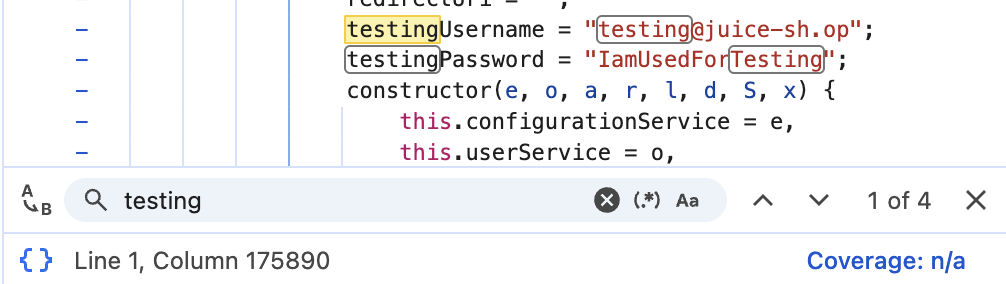
\includegraphics[width=0.5\textwidth]{images/2-3.png}
    \caption{在 main.js 中找到的帳號密碼}
    \label{fig:2-3}
  \end{figure}
\end{enumerate}

\subsubsection*{Scoreboard 截圖：}
\begin{figure}[H]
  \centering
  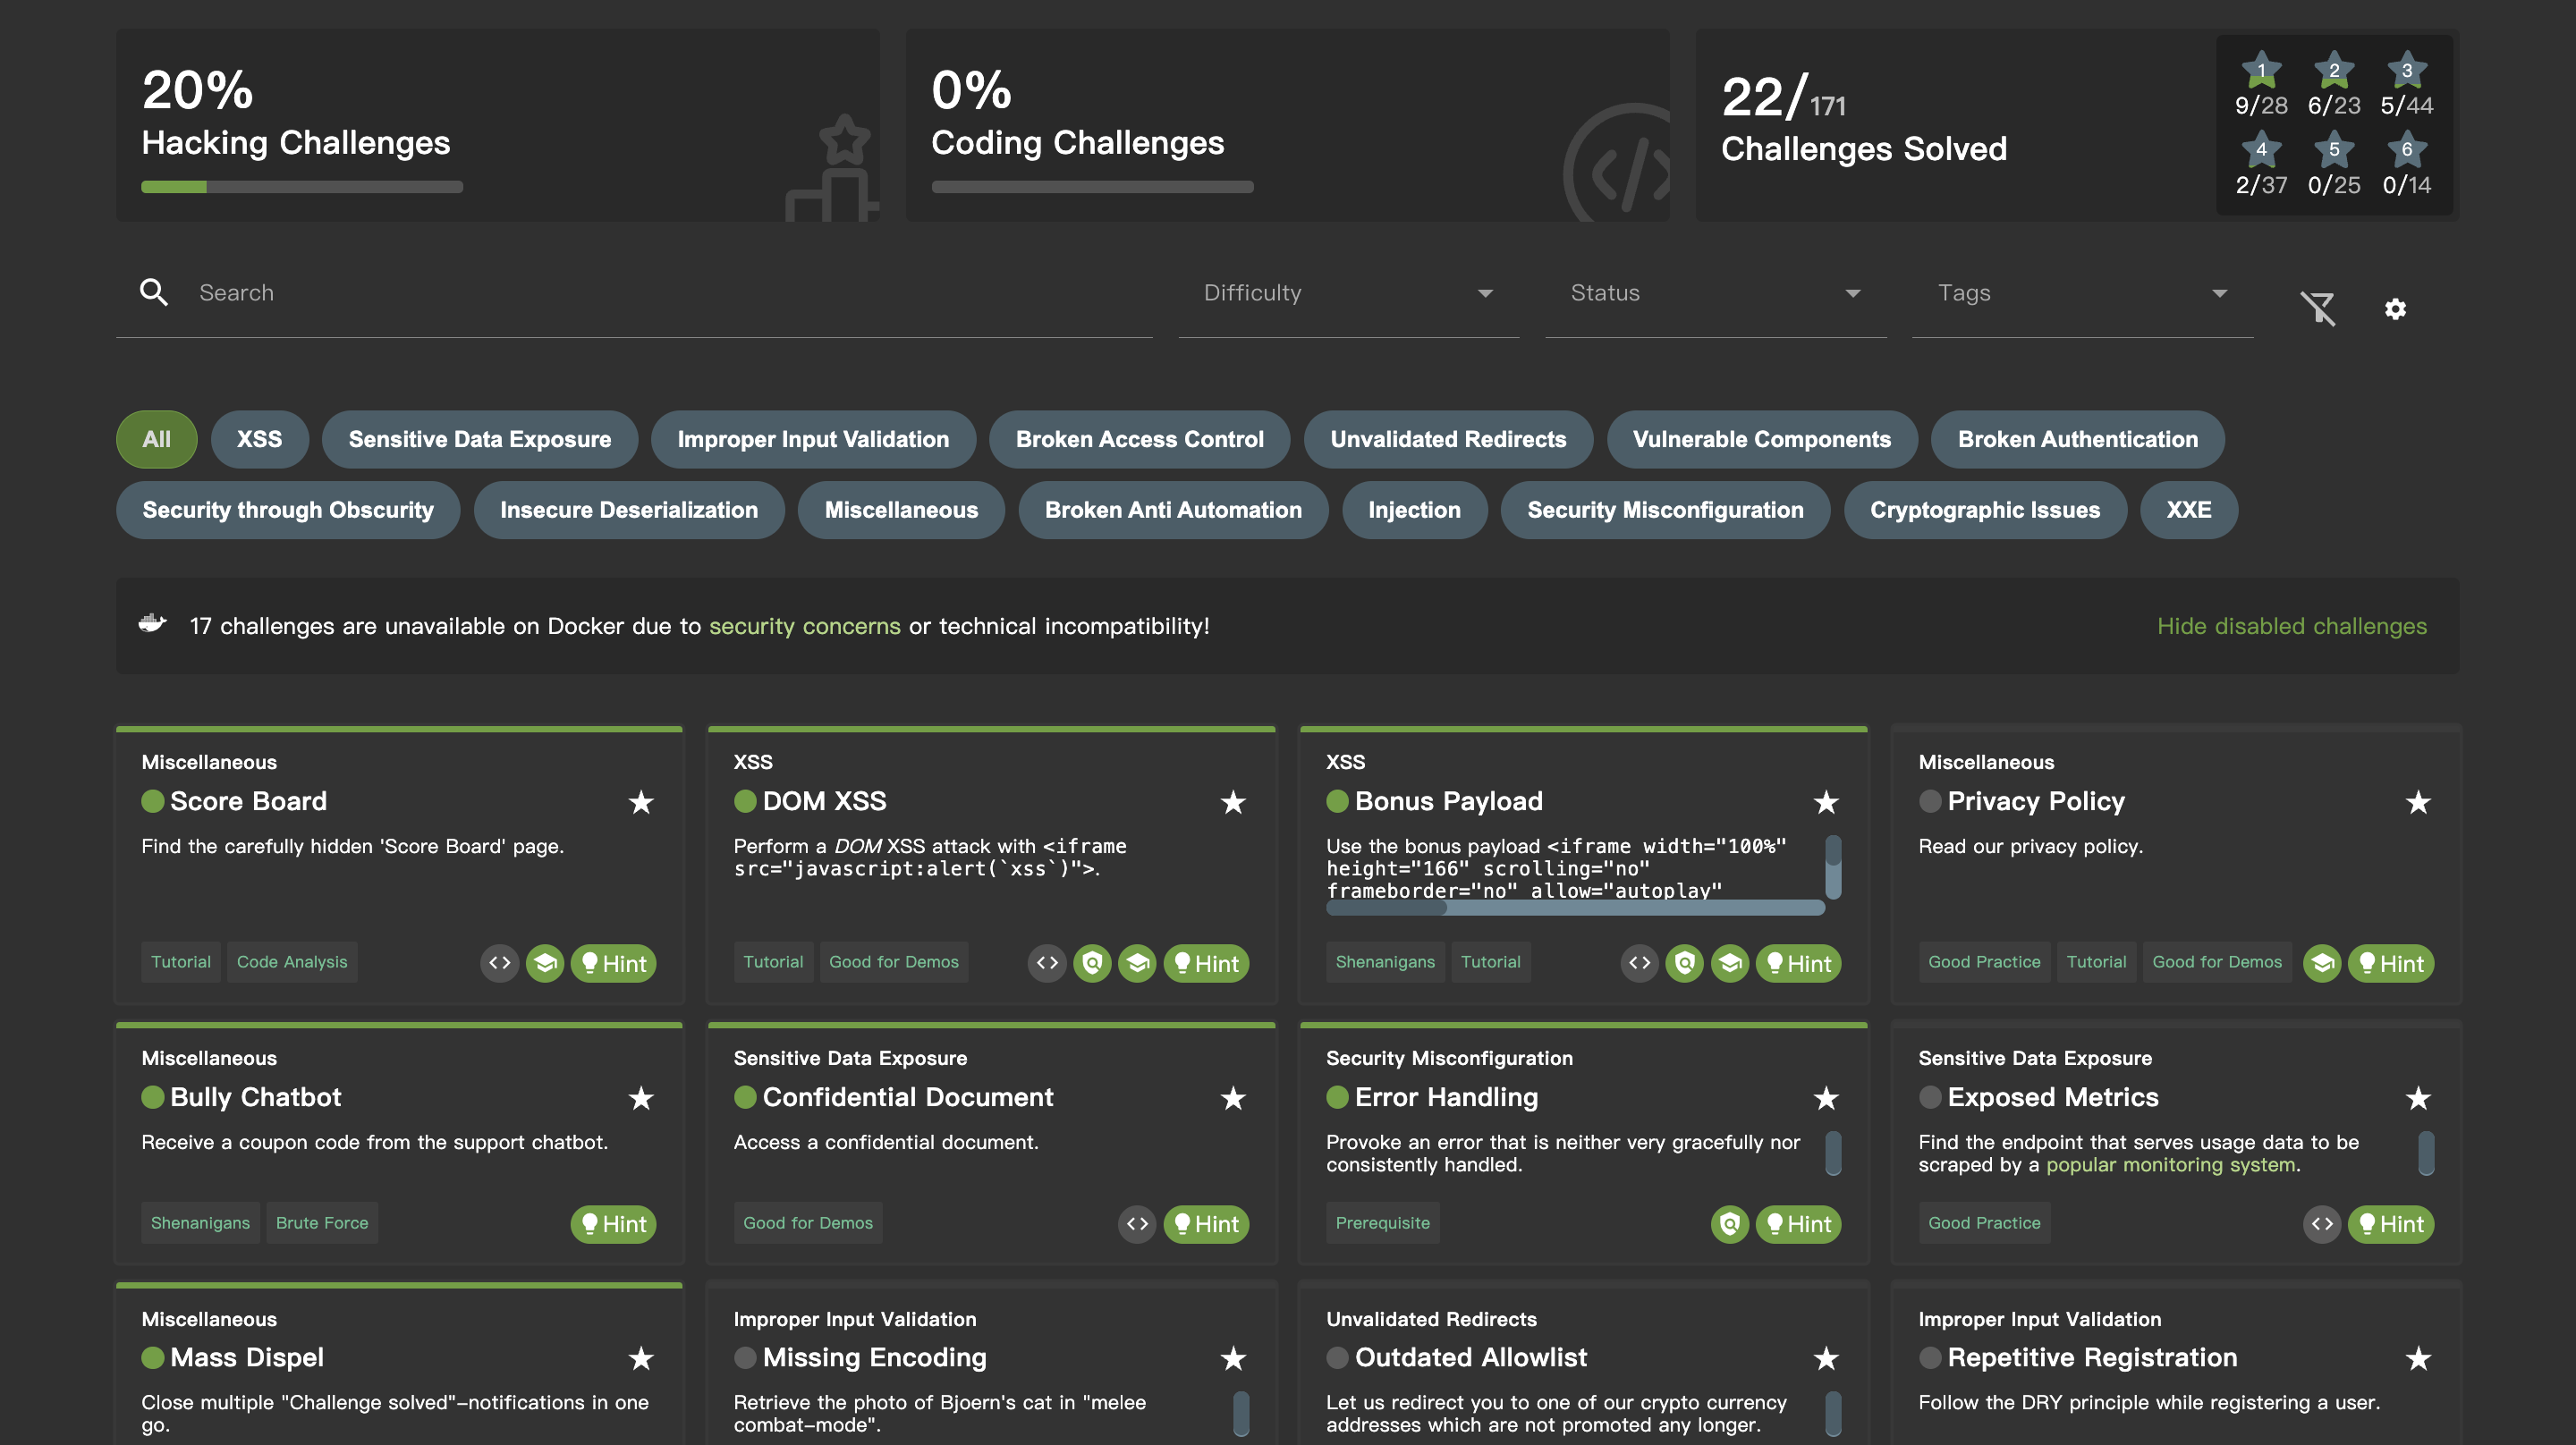
\includegraphics[width=\textwidth]{images/2-4.png}
  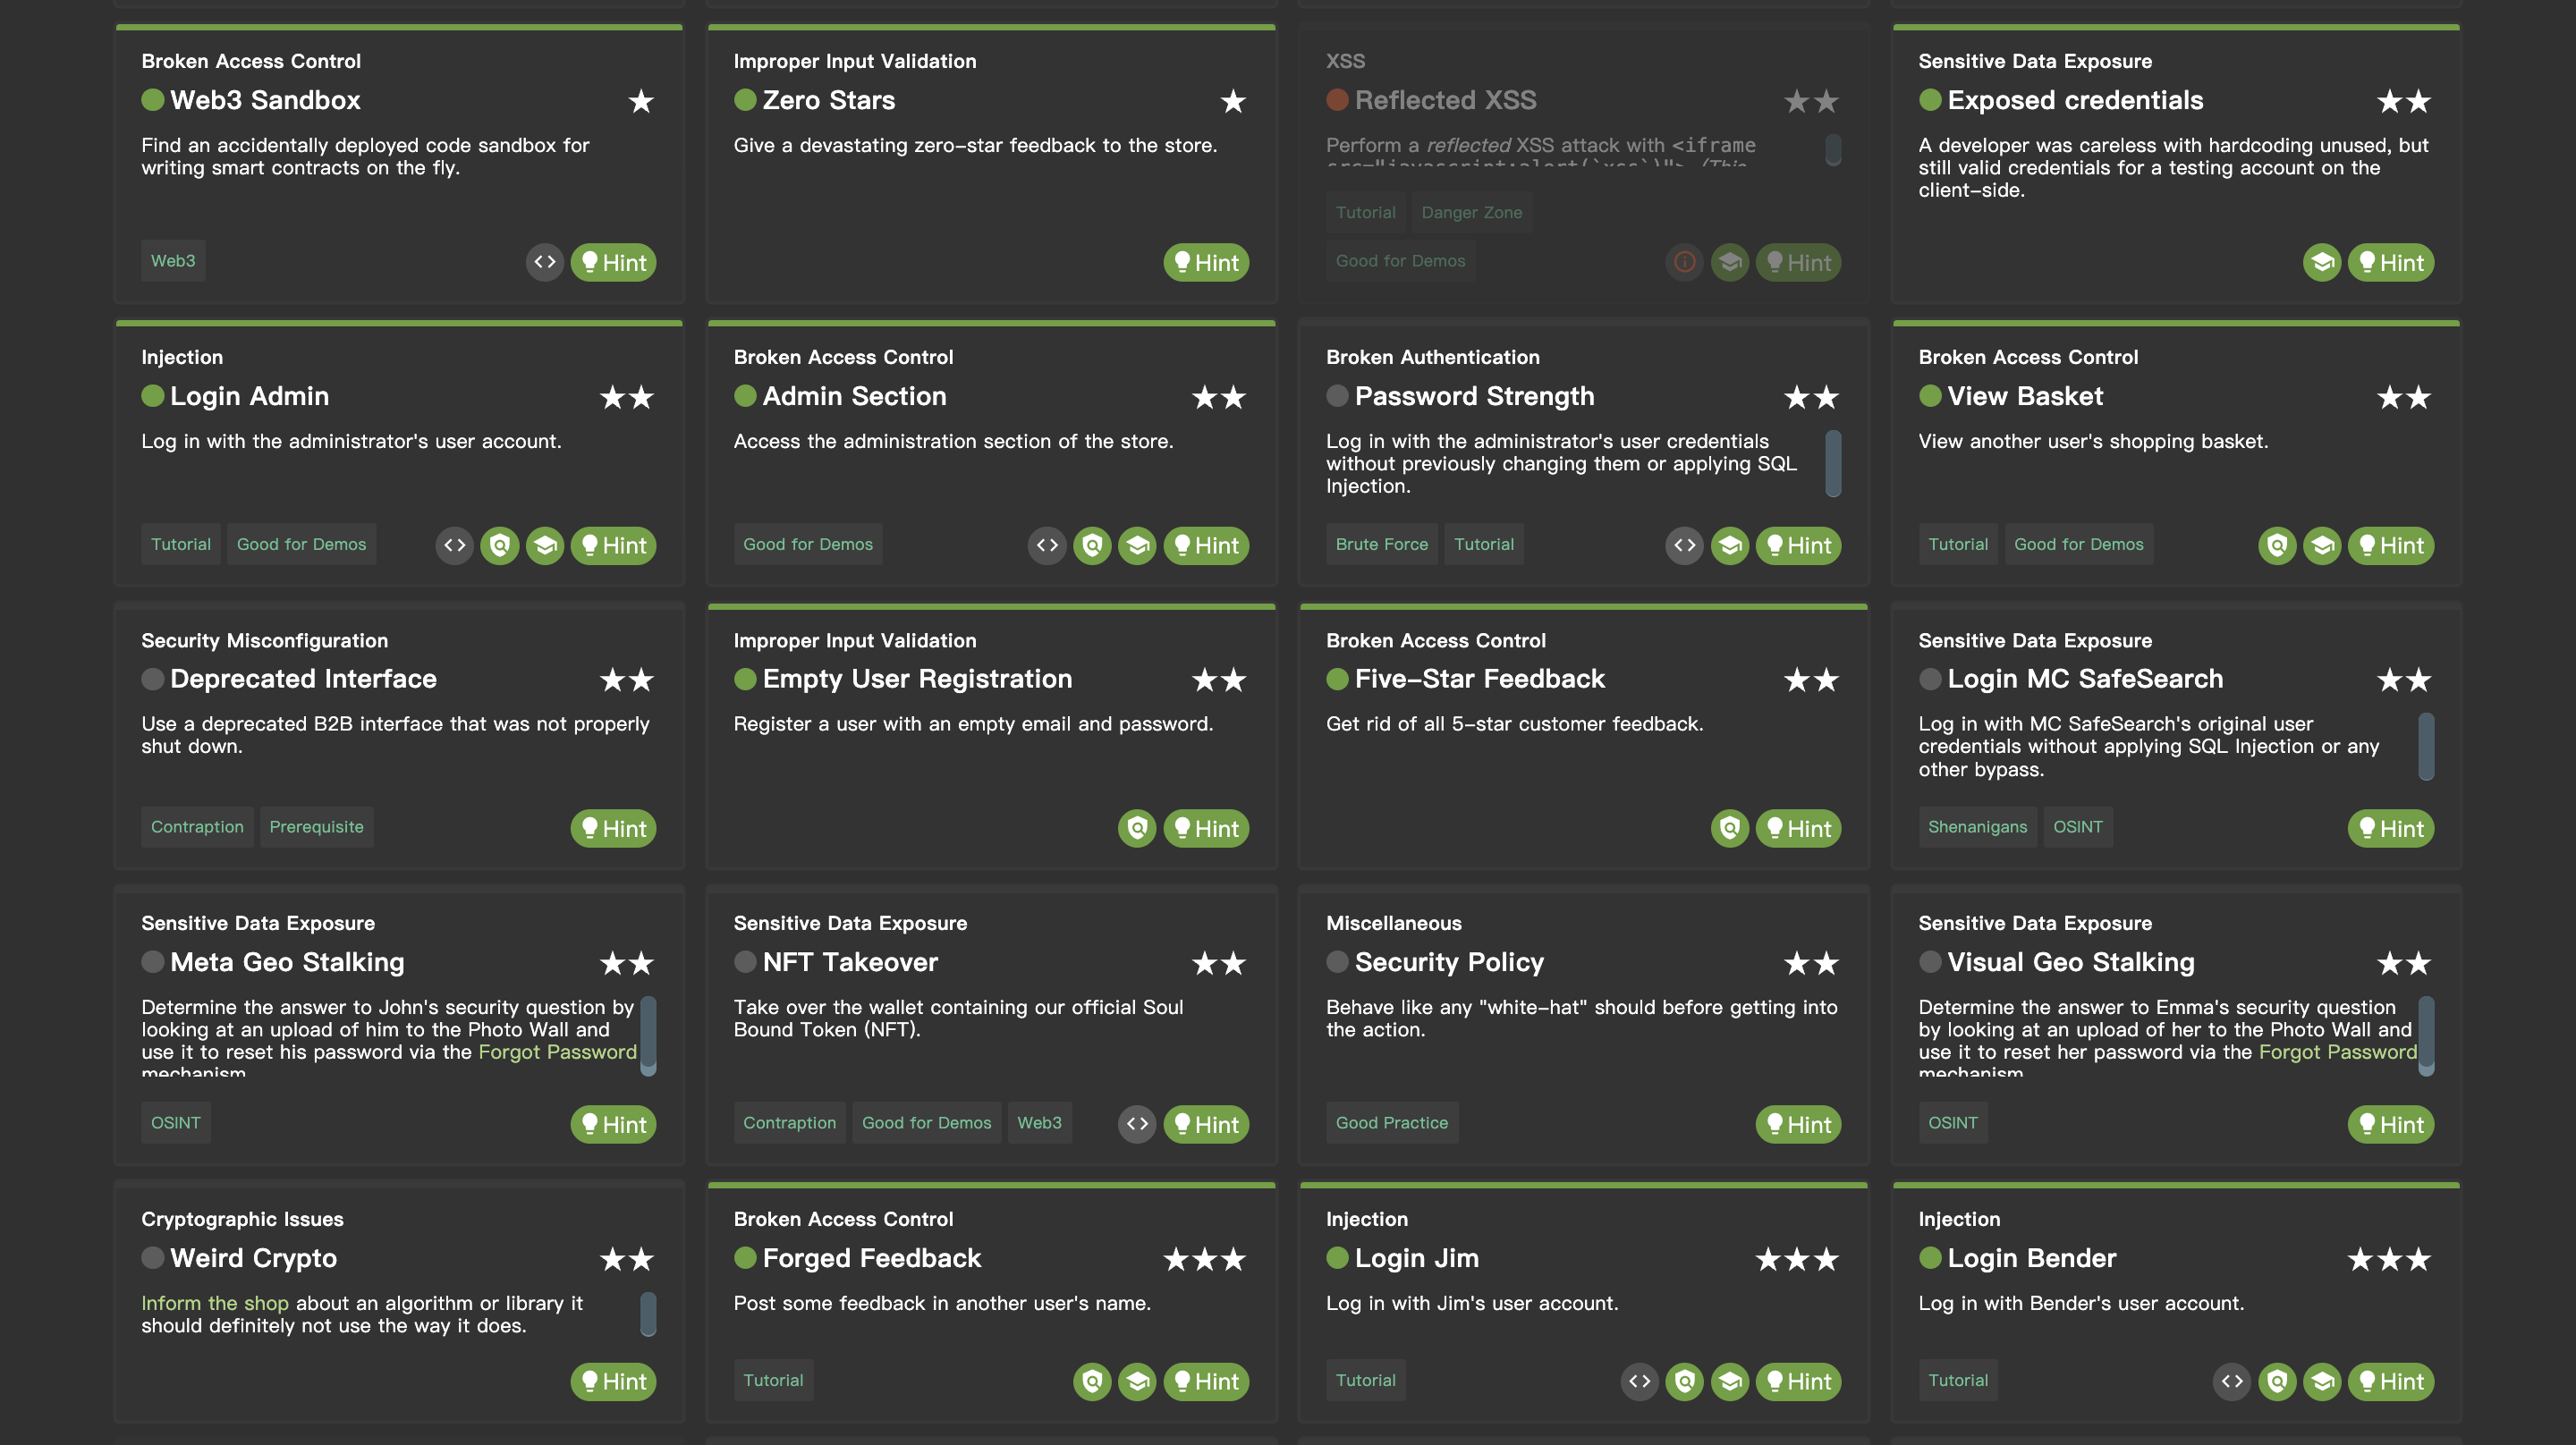
\includegraphics[width=\textwidth]{images/2-5.png}
  \caption{Juice Shop 的 Scoreboard}
  \label{fig:2-4}
\end{figure}

\clearpage
\subsection{SSRF、CSRF 和 XSS}
\begin{itemize}
  \item \textbf{SSRF（Server-Side Request Forgery）:}

  在這種攻擊方式中，攻擊者利用伺服器端的向特定的另一個服務發送請求，通常是為了繞過防火牆或存取內部網路資源。常見的情況是，假如你的網站上有個輸入框，讓使用者自己填網址。攻擊者就可以偷偷填一個公司內網的地址，讓你的伺服器去「自動」幫他連過去。結果可能拿到內網機密、撈到不該給外部看的資料，甚至繞過防火牆去搞其他事。

  \item \textbf{CSRF（Cross-Site Request Forgery）:}

  在這種攻擊中，攻擊者誘使使用者在已經登入的情況下，透過攻擊者先在別的網站或郵件裡夾一個隱藏的請求連結，發送未經授權的請求到另一個網站。只要你正好在同一瀏覽器裡已經登入了某個網站，瀏覽器就會帶上你的 Cookie／驗證資訊，自動幫你送出那個請求，並用你的身份執行操作。結果你可能就被偷轉帳、改設定或亂發文。

  \item \textbf{XSS（Cross-Site Scripting）:}
  
  基本上，攻擊者把惡意 JavaScript 或 HTML 混進你信任的網頁裡，等人一打開網頁，腳本就在使用者的瀏覽器跑起來。可以偷 Cookie、竊取表單資料，甚至直接在頁面上做釣魚操作。

  \item \textbf{三者比較:} 
  \begin{table}[H]
    \centering
    \begin{tabular}{p{2cm}ccc}
      \toprule
      \textbf{攻擊類型} & \textbf{SSRF} & \textbf{CSRF} & \textbf{XSS} \\
      \midrule
      \textbf{攻擊對象} & 伺服器 & 使用者 & 使用者 \\
      \textbf{攻擊方式} & 利用伺服器發送請求 & 誘使使用者發送請求 & 注入惡意腳本 \\
      \textbf{影響範圍} & 伺服器內部資源 & 使用者帳號 & 使用者瀏覽器 \\
      \bottomrule
    \end{tabular}
    \caption{SSRF、CSRF 和 XSS 的比較}
    \label{tab:ssrf-csrf-xss}
  \end{table}
\end{itemize}


% ------------------------------------------------------------
% Problem 3 (30 points)
% ------------------------------------------------------------
\section{R-SA！破密部}



% ------------------------------------------------------------
% Problem 4 (41 points)
% ------------------------------------------------------------
\clearpage
\section{TESTING in the FUZZ}

% ------------------------------------------------------------
% Problem 5 (28 points)
% ------------------------------------------------------------
\clearpage
\section{敗北協定太多了！}

% ------------------------------------------------------------
% Problem 6 (34 points)
% ------------------------------------------------------------
\clearpage
\section{猫物語（赤）}



% -----------------------------------------------------------
%    You don't have to mess with anything below this line.
% -----------------------------------------------------------

\end{document}
